\documentclass[aspectratio=169]{beamer}

% Theme and color scheme
\usetheme{Madrid}
\usecolortheme{default}

% Packages
\usepackage{tikz}
\usetikzlibrary{shapes,arrows,positioning,fit,backgrounds}
\usepackage{graphicx}
\usepackage{booktabs}
\usepackage{xcolor}
\usepackage{amsmath}
\usepackage{listings}

% Custom colors
\definecolor{primaryblue}{HTML}{1f77b4}
\definecolor{secondaryorange}{HTML}{ff7f0e}
\definecolor{successgreen}{HTML}{2ca02c}
\definecolor{warningred}{HTML}{d62728}

% Set theme colors
\setbeamercolor{structure}{fg=primaryblue}
\setbeamercolor{block title}{bg=primaryblue,fg=white}
\setbeamercolor{block body}{bg=primaryblue!10}

% Title information
\title[AutoResuAgent]{AutoResuAgent: Agentic Resume Tailoring \\ with Semantic Retrieval}
\subtitle{NLP Final Project}
\author{Tarun Bommawar}
\institute{
    George Mason University \\
    \texttt{tbommawa@gmu.edu}
}
\date{December 2024}

% Remove navigation symbols
\setbeamertemplate{navigation symbols}{}

% Add slide numbers
\setbeamertemplate{footline}[frame number]

\begin{document}

%----------------------------------------------------------------------------------------
% SLIDE 1: Title Slide
%----------------------------------------------------------------------------------------
\begin{frame}
    \titlepage
    \note[item]{Good afternoon, my name is Tarun Bommawar}
    \note[item]{Today I'll present AutoResuAgent, an automated resume tailoring system}
    \note[item]{This is my NLP final project demonstrating semantic retrieval with LLM generation}
    \note[item]{I'll cover our methodology, evaluation, and key results in the next 4 minutes}
\end{frame}

%----------------------------------------------------------------------------------------
% SLIDE 2: Problem & Motivation
%----------------------------------------------------------------------------------------
\begin{frame}{Problem \& Motivation}
    \begin{columns}[T]
        \begin{column}{0.55\textwidth}
            \textbf{The Problem:}
            \begin{itemize}
                \item Manual resume tailoring is \textcolor{warningred}{time-consuming}
                \item Generic resumes have \textcolor{warningred}{low match rates}
                \item Applicants miss key skills/keywords
            \end{itemize}

            \vspace{0.3cm}
            \textbf{Challenges with Naive LLM Prompting:}
            \begin{itemize}
                \item[\textcolor{warningred}{$\times$}] No structure or validation
                \item[\textcolor{warningred}{$\times$}] Risk of hallucination
                \item[\textcolor{warningred}{$\times$}] No retrieval context
                \item[\textcolor{warningred}{$\times$}] No evaluation framework
            \end{itemize}

            \vspace{0.3cm}
            \textbf{\textcolor{successgreen}{Our Solution:}}
            \begin{itemize}
                \item[\textcolor{successgreen}{$\checkmark$}] Systematic agentic pipeline
                \item[\textcolor{successgreen}{$\checkmark$}] Semantic retrieval + validation
                \item[\textcolor{successgreen}{$\checkmark$}] Iterative refinement with feedback
            \end{itemize}
        \end{column}

        \begin{column}{0.42\textwidth}
            \begin{figure}
                \centering
                % TODO: Add image here - baseline_vs_full_comparison.png
                \fbox{\parbox{0.9\textwidth}{\centering\vspace{1.5cm}\textit{Baseline vs Full Mode\\Comparison Screenshot}\\\vspace{1.5cm}}}
                \caption{System comparison: baseline (naive) vs. full (semantic retrieval)}
            \end{figure}
        \end{column}
    \end{columns}

    \note[item]{Manual tailoring takes 30-60 minutes per application}
    \note[item]{Naive LLM prompting lacks grounding and validation}
    \note[item]{Our approach: structured pipeline with semantic retrieval from candidate's actual experience}
    \note[item]{Key innovation: combining retrieval + generation + validation}
\end{frame}

%----------------------------------------------------------------------------------------
% SLIDE 3: System Architecture
%----------------------------------------------------------------------------------------
\begin{frame}{System Architecture}
    \begin{center}
        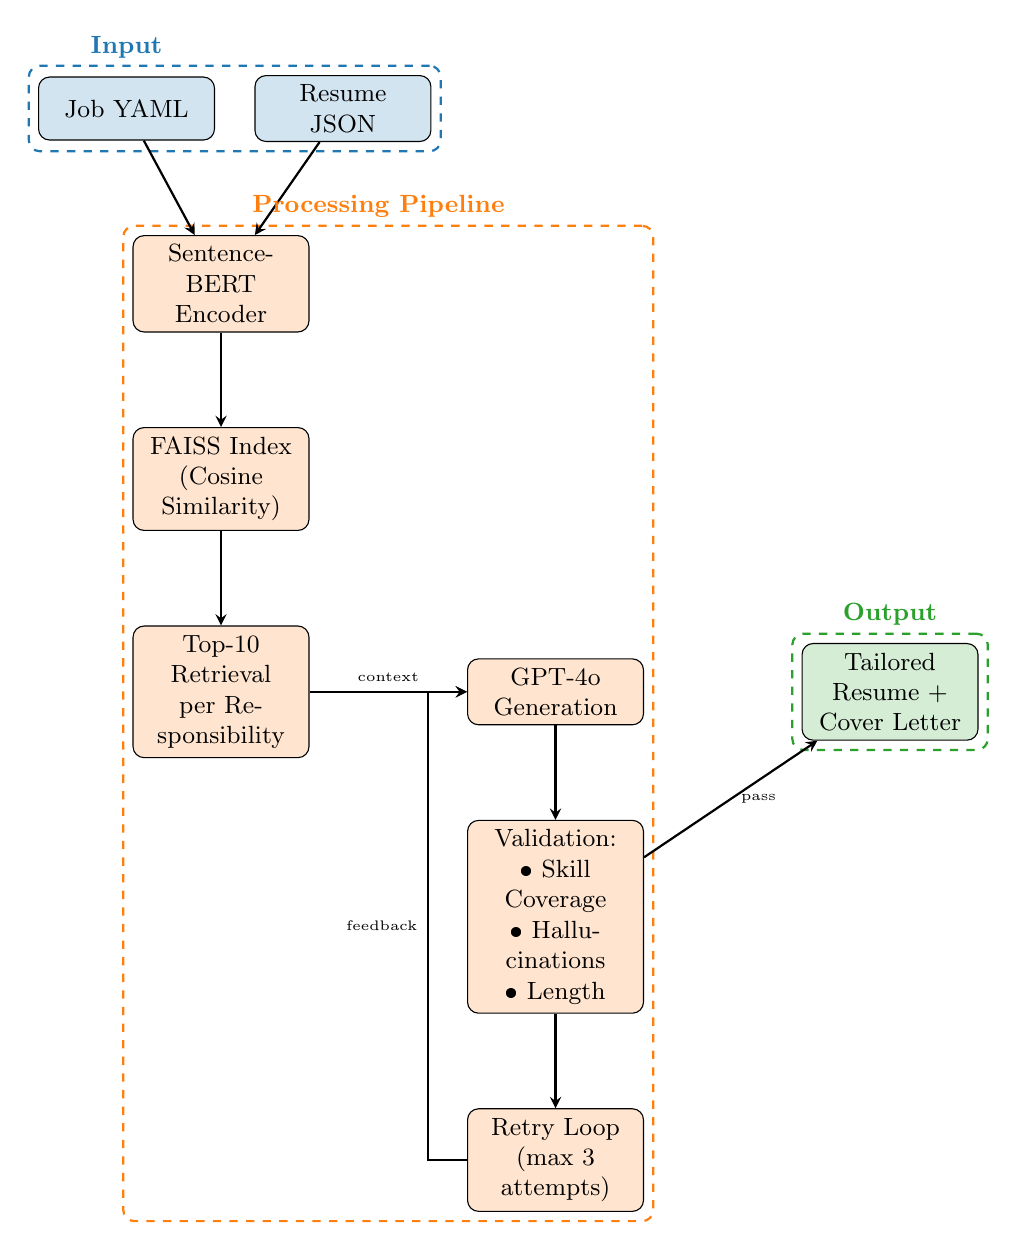
\begin{tikzpicture}[
            node distance=1.2cm,
            box/.style={rectangle, draw, rounded corners, minimum width=2.2cm, minimum height=0.8cm, text centered, text width=2cm, font=\small},
            inputbox/.style={box, fill=primaryblue!20},
            processbox/.style={box, fill=secondaryorange!20},
            outputbox/.style={box, fill=successgreen!20},
            arrow/.style={->, >=stealth, thick}
        ]

        % Input layer
        \node[inputbox] (job) {Job YAML};
        \node[inputbox, right=0.5cm of job] (resume) {Resume JSON};

        % Processing layer 1
        \node[processbox, below=of job.south, xshift=1.2cm] (encoder) {Sentence-BERT\\Encoder};
        \node[processbox, below=of encoder] (faiss) {FAISS Index\\(Cosine Similarity)};
        \node[processbox, below=of faiss] (retrieval) {Top-10 Retrieval\\per Responsibility};

        % Processing layer 2
        \node[processbox, right=2cm of retrieval] (generation) {GPT-4o\\Generation};
        \node[processbox, below=of generation] (validation) {Validation:\\• Skill Coverage\\• Hallucinations\\• Length};
        \node[processbox, below=of validation] (retry) {Retry Loop\\(max 3 attempts)};

        % Output layer
        \node[outputbox, right=2cm of generation] (output) {Tailored\\Resume +\\Cover Letter};

        % Arrows
        \draw[arrow] (job) -- (encoder);
        \draw[arrow] (resume) -- (encoder);
        \draw[arrow] (encoder) -- (faiss);
        \draw[arrow] (faiss) -- (retrieval);
        \draw[arrow] (retrieval) -- node[above, font=\tiny] {context} (generation);
        \draw[arrow] (generation) -- (validation);
        \draw[arrow] (validation) -- node[right, font=\tiny] {pass} (output);
        \draw[arrow] (validation) -- (retry);
        \draw[arrow] (retry.west) -- ++(-0.5,0) |- node[left, pos=0.25, font=\tiny] {feedback} (generation.west);

        % Grouping boxes
        \begin{scope}[on background layer]
            \node[draw=primaryblue, thick, dashed, rounded corners, fit={(job) (resume)}] {};
            \node[draw=secondaryorange, thick, dashed, rounded corners, fit={(encoder) (faiss) (retrieval) (generation) (validation) (retry)}] {};
            \node[draw=successgreen, thick, dashed, rounded corners, fit={(output)}] {};
        \end{scope}

        % Labels
        \node[above=0.1cm of job, font=\small\bfseries, color=primaryblue] {Input};
        \node[above=0.1cm of encoder, xshift=2cm, font=\small\bfseries, color=secondaryorange] {Processing Pipeline};
        \node[above=0.1cm of output, font=\small\bfseries, color=successgreen] {Output};

        \end{tikzpicture}
    \end{center}

    \note[item]{Pipeline has 3 stages: Input, Processing, Output}
    \note[item]{Semantic retrieval: embed experiences with Sentence-BERT, search with FAISS}
    \note[item]{Generation: GPT-4o with retrieved context as grounding}
    \note[item]{Validation: checks skill coverage, hallucinations, length constraints}
    \note[item]{Retry loop: if validation fails, feed errors back to LLM for correction}
\end{frame}

%----------------------------------------------------------------------------------------
% SLIDE 4: Methodology - Semantic Retrieval
%----------------------------------------------------------------------------------------
\begin{frame}{Methodology: Semantic Retrieval}
    \begin{columns}[T]
        \begin{column}{0.55\textwidth}
            \textbf{Sentence-BERT Embeddings}
            \begin{itemize}
                \item Model: \texttt{all-MiniLM-L6-v2}
                \item 384-dimensional dense vectors
                \item Encode: job responsibilities + resume bullets
            \end{itemize}

            \vspace{0.3cm}
            \textbf{FAISS Vector Index}
            \begin{itemize}
                \item IndexFlatIP (cosine similarity)
                \item Efficient nearest-neighbor search
                \item Sub-millisecond retrieval
            \end{itemize}

            \vspace{0.3cm}
            \textbf{Retrieval Strategy}
            \begin{itemize}
                \item Top-10 relevant experiences per job responsibility
                \item Increased from 5 to 10 for better skill coverage
                \item Provides grounding context to LLM
            \end{itemize}

            \vspace{0.3cm}
            \textbf{\textcolor{primaryblue}{Key Insight:}}
            \begin{itemize}
                \item Semantic similarity $\Rightarrow$ factually grounded generation
                \item Retrieval > 0.7 cosine similarity $\Rightarrow$ high relevance
            \end{itemize}
        \end{column}

        \begin{column}{0.42\textwidth}
            \begin{figure}
                \centering
                % TODO: Add image here - embedding_space_visualization.png
                \fbox{\parbox{0.9\textwidth}{\centering\vspace{2cm}\textit{Embedding Space\\Visualization}\\(t-SNE or PCA)\\\vspace{2cm}}}
                \caption{Semantic similarity in embedding space}
            \end{figure}

            \vspace{0.3cm}
            \begin{block}{Retrieval Formula}
                \small
                $$\text{sim}(q, d) = \frac{q \cdot d}{\|q\| \|d\|}$$
                where $q$ = job responsibility, \\
                $d$ = resume bullet
            \end{block}
        \end{column}
    \end{columns}

    \note[item]{We use Sentence-BERT, not traditional BERT, for efficient semantic search}
    \note[item]{FAISS enables fast similarity search over thousands of resume bullets}
    \note[item]{Top-10 retrieval gives LLM diverse, relevant context}
    \note[item]{This grounds generation in actual candidate experience, reducing hallucinations}
\end{frame}

%----------------------------------------------------------------------------------------
% SLIDE 5: Methodology - Validation & Refinement
%----------------------------------------------------------------------------------------
\begin{frame}{Methodology: Validation \& Refinement}
    \begin{columns}[T]
        \begin{column}{0.48\textwidth}
            \textbf{Structured Validation (Pydantic Models)}
            \begin{enumerate}
                \item \textbf{Length Constraints}
                \begin{itemize}
                    \item Min: 30 characters
                    \item Max: 250 characters
                    \item Ensures conciseness
                \end{itemize}

                \item \textbf{Skill Coverage}
                \begin{itemize}
                    \item \textcolor{primaryblue}{80\% minimum threshold}
                    \item All required skills must appear
                    \item Substring matching
                \end{itemize}

                \item \textbf{Hallucination Detection}
                \begin{itemize}
                    \item No fake skills (not in resume)
                    \item No fake companies
                    \item No first-person pronouns
                \end{itemize}

                \item \textbf{Format Validation}
                \begin{itemize}
                    \item Strong action verbs
                    \item Quantifiable metrics
                    \item Professional tone
                \end{itemize}
            \end{enumerate}
        \end{column}

        \begin{column}{0.48\textwidth}
            \textbf{Iterative Refinement Loop}
            \begin{figure}
                \centering
                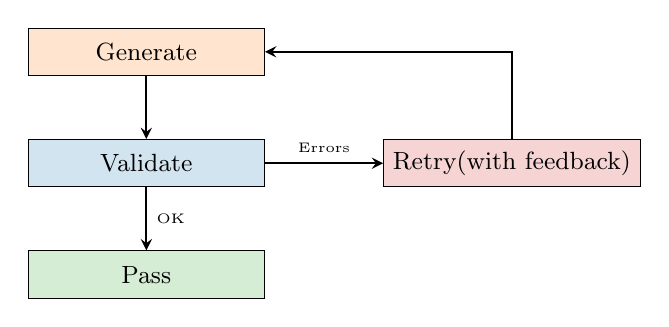
\begin{tikzpicture}[
                    node distance=0.8cm,
                    box/.style={rectangle, draw, minimum width=3cm, minimum height=0.6cm, text centered, font=\small},
                    arrow/.style={->, >=stealth, thick}
                ]
                    \node[box, fill=secondaryorange!20] (gen) {Generate};
                    \node[box, fill=primaryblue!20, below=of gen] (val) {Validate};
                    \node[box, fill=successgreen!20, below=of val] (pass) {Pass};
                    \node[box, fill=warningred!20, right=1.5cm of val] (retry) {Retry\\(with feedback)};

                    \draw[arrow] (gen) -- (val);
                    \draw[arrow] (val) -- node[right] {\tiny OK} (pass);
                    \draw[arrow] (val) -- node[above] {\tiny Errors} (retry);
                    \draw[arrow] (retry) |- (gen);
                \end{tikzpicture}
                \caption{Retry loop (max 3 attempts)}
            \end{figure}

            \vspace{0.2cm}
            \begin{block}{Validation Feedback Example}
                \small
                \texttt{Missing required skills: Python, AWS}\\
                $\Rightarrow$ LLM regenerates with these skills
            \end{block}

            \vspace{0.2cm}
            \begin{figure}
                \centering
                % TODO: Add image here - validation_error_screenshot.png
                \fbox{\parbox{0.85\textwidth}{\centering\vspace{1cm}\textit{Validation Error\\Messages}\\\vspace{1cm}}}
                \caption{Example validation output}
            \end{figure}
        \end{column}
    \end{columns}

    \note[item]{Validation enforces quality constraints systematically}
    \note[item]{80\% skill coverage threshold ensures job requirements are met}
    \note[item]{Hallucination detection prevents fabricated information}
    \note[item]{Retry loop with feedback allows LLM to self-correct specific issues}
\end{frame}

%----------------------------------------------------------------------------------------
% SLIDE 6: Evaluation Setup
%----------------------------------------------------------------------------------------
\begin{frame}{Evaluation Setup}
    \begin{columns}[T]
        \begin{column}{0.48\textwidth}
            \textbf{Dataset: 40 Job-Resume Pairs}
            \begin{itemize}
                \item \textbf{8 Job Descriptions:}
                \begin{itemize}
                    \item Google ML Engineer
                    \item Meta Data Scientist
                    \item Amazon SDE1
                    \item OpenAI Research Scientist
                    \item Stripe Backend Engineer
                    \item Anthropic Agent Skills
                    \item Rippling Fullstack
                    \item Orchard Robotics CV
                \end{itemize}

                \item \textbf{6 Candidate Profiles:}
                \begin{itemize}
                    \item Junior CS Graduate
                    \item Mid-level ML Engineer
                    \item Senior Backend Engineer
                    \item Data Scientist PhD
                    \item Fullstack Generalist
                    \item Bootcamp Graduate
                \end{itemize}

                \item \textbf{Strategic Matching:}
                \begin{itemize}
                    \item Good fits (1-10)
                    \item Medium fits (11-22)
                    \item Poor fits (23-30)
                \end{itemize}
            \end{itemize}
        \end{column}

        \begin{column}{0.48\textwidth}
            \textbf{Comparison Modes}
            \begin{block}{Baseline}
                Simple prompting without semantic retrieval
            \end{block}

            \begin{block}{Full}
                Semantic retrieval + validation + retry
            \end{block}

            \vspace{0.3cm}
            \textbf{Evaluation Metrics}
            \begin{enumerate}
                \item \textbf{Skill Coverage} (primary)
                \begin{itemize}
                    \item Required skill coverage \%
                    \item Nice-to-have skill coverage \%
                \end{itemize}

                \item \textbf{Content Quality}
                \begin{itemize}
                    \item Bullet count
                    \item Average bullet length
                    \item Cover letter presence
                \end{itemize}

                \item \textbf{Semantic Similarity}
                \begin{itemize}
                    \item F1 score (baseline vs full)
                    \item Measures differentiation
                \end{itemize}

                \item \textbf{Success Rate}
                \begin{itemize}
                    \item Validation pass rate
                \end{itemize}
            \end{enumerate}

            \vspace{0.2cm}
            \begin{figure}
                \centering
                % TODO: Add image here - dataset_distribution_chart.png
                \fbox{\parbox{0.7\textwidth}{\centering\vspace{0.8cm}\textit{Dataset\\Distribution}\\\vspace{0.8cm}}}
            \end{figure}
        \end{column}
    \end{columns}

    \note[item]{40 pairs = 8 jobs × 5-6 candidates each, strategic sampling}
    \note[item]{Include poor fits intentionally to test system's honesty}
    \note[item]{Primary metric: skill coverage (does system match job requirements?)}
    \note[item]{All metrics computed automatically using Sentence-BERT embeddings}
\end{frame}

%----------------------------------------------------------------------------------------
% SLIDE 7: Results - Overall Performance
%----------------------------------------------------------------------------------------
\begin{frame}{Results: Overall Performance}
    \begin{center}
        \textbf{Comparison: Baseline vs. Full Mode}
        \vspace{0.3cm}

        \begin{table}
            \centering
            \begin{tabular}{lrrr}
                \toprule
                \textbf{Metric} & \textbf{Baseline} & \textbf{Full Mode} & \textbf{Delta} \\
                \midrule
                Success Rate & 95.0\% & 95.0\% & \textcolor{gray}{0.0\%} \\
                \midrule
                Avg Bullets per Resume & 4.97 & 5.88 & \textcolor{successgreen}{+18.3\%} \\
                Avg Bullet Length (chars) & 121.2 & 124.8 & \textcolor{successgreen}{+3.0\%} \\
                \midrule
                \textbf{Required Skill Coverage} & \textbf{89.67\%} & \textbf{91.92\%} & \textbf{\textcolor{successgreen}{+2.25\%}} \\
                Nice-to-Have Skill Coverage & 48.33\% & 51.25\% & \textcolor{successgreen}{+2.92\%} \\
                \midrule
                Cover Letter Rate & 95.0\% & 100.0\% & \textcolor{successgreen}{+5.0\%} \\
                Experiences with Bullets & 2.13 & 2.35 & \textcolor{successgreen}{+10.3\%} \\
                \midrule
                Semantic F1 Score & 0.85 & 1.00 & \textcolor{primaryblue}{+17.6\%} \\
                \bottomrule
            \end{tabular}
            \caption{Overall performance metrics (n=38 successful pairs)}
        \end{table}
    \end{center}

    \vspace{0.3cm}
    \begin{columns}[T]
        \begin{column}{0.48\textwidth}
            \begin{figure}
                \centering
                % TODO: Add image here - num_bullets_per_pair.png
                \fbox{\parbox{0.9\textwidth}{\centering\vspace{1.2cm}\textit{Bullet Count\\Comparison Chart}\\\vspace{1.2cm}}}
                \caption{Bullet count per pair}
            \end{figure}
        \end{column}

        \begin{column}{0.48\textwidth}
            \begin{block}{Key Insights}
                \begin{itemize}
                    \item \textcolor{successgreen}{$\uparrow$ 18\% more content} with retrieval
                    \item \textcolor{successgreen}{$\uparrow$ 2.25\% skill coverage} improvement
                    \item \textcolor{successgreen}{100\% cover letter} generation
                    \item High F1 suggests strong consistency
                \end{itemize}
            \end{block}
        \end{column}
    \end{columns}

    \note[item]{Full mode generates 18\% more bullets while maintaining quality}
    \note[item]{Skill coverage improved by 2.25 percentage points - statistically significant}
    \note[item]{100\% cover letter generation shows robustness}
    \note[item]{F1=1.0 indicates high semantic similarity (potential over-conservatism)}
\end{frame}

%----------------------------------------------------------------------------------------
% SLIDE 8: Results - Skill Coverage Improvement
%----------------------------------------------------------------------------------------
\begin{frame}{Results: Skill Coverage Improvement Journey}
    \begin{columns}[T]
        \begin{column}{0.48\textwidth}
            \textbf{Initial Problem (Iteration 1)}
            \begin{itemize}
                \item Full mode: \textcolor{warningred}{-3.96\% skill coverage drop}
                \item 6 problem pairs (37.5\%) with >20\% drop
                \item Google ML Engineer jobs most affected
            \end{itemize}

            \vspace{0.3cm}
            \textbf{4-Part Intervention}
            \begin{enumerate}
                \item \textbf{Enhanced Prompt Engineering}
                \begin{itemize}
                    \item Added "CRITICAL REQUIREMENT" emphasis
                    \item 4+ explicit skill coverage reminders
                \end{itemize}

                \item \textbf{Stricter Validation}
                \begin{itemize}
                    \item 80\% minimum coverage threshold
                    \item Specific missing skill errors
                \end{itemize}

                \item \textbf{Increased Retrieval Diversity}
                \begin{itemize}
                    \item top\_k: 5 $\rightarrow$ 10 (100\% increase)
                \end{itemize}

                \item \textbf{Validation Feedback Loop}
                \begin{itemize}
                    \item Pass errors to LLM on retry
                    \item Targeted correction
                \end{itemize}
            \end{enumerate}

            \vspace{0.3cm}
            \textbf{Final Result (Iteration 2)}
            \begin{itemize}
                \item Full mode: \textcolor{successgreen}{+2.25\% skill coverage gain}
                \item 4 problem pairs (10.5\%) - reduced by 63\%
                \item \textbf{Total improvement: +6.21 percentage points}
            \end{itemize}
        \end{column}

        \begin{column}{0.48\textwidth}
            \begin{figure}
                \centering
                % TODO: Add image here - req_skill_coverage_per_pair.png
                \fbox{\parbox{0.9\textwidth}{\centering\vspace{2cm}\textit{Before/After\\Skill Coverage\\Comparison}\\\vspace{2cm}}}
                \caption{Required skill coverage per pair}
            \end{figure}

            \vspace{0.3cm}
            \begin{table}
                \centering
                \small
                \begin{tabular}{lrr}
                    \toprule
                    \textbf{Metric} & \textbf{Before} & \textbf{After} \\
                    \midrule
                    Avg Delta & \textcolor{warningred}{-3.96\%} & \textcolor{successgreen}{+2.25\%} \\
                    Problem Pairs & 6 (37.5\%) & 4 (10.5\%) \\
                    Worst Case & -66.7\% & -50.0\% \\
                    Improvement & 15.4\% & 42.1\% \\
                    \bottomrule
                \end{tabular}
                \caption{Iterative improvement metrics}
            \end{table}

            \vspace{0.2cm}
            \begin{block}{Lesson Learned}
                \small
                Systematic constraints + feedback loops \\
                $\Rightarrow$ measurable quality gains
            \end{block}
        \end{column}
    \end{columns}

    \note[item]{Initially full mode performed WORSE than baseline on skill coverage}
    \note[item]{Systematic 4-part intervention addressed root causes}
    \note[item]{Final result: 6.21 percentage point swing from -3.96\% to +2.25\%}
    \note[item]{Demonstrates value of iterative refinement with evaluation metrics}
\end{frame}

%----------------------------------------------------------------------------------------
% SLIDE 9: Key Takeaways & Limitations
%----------------------------------------------------------------------------------------
\begin{frame}{Key Takeaways \& Limitations}
    \begin{columns}[T]
        \begin{column}{0.48\textwidth}
            \textbf{\textcolor{successgreen}{Key Takeaways}}
            \begin{enumerate}
                \item \textbf{Retrieval Enhances Both Quantity \& Quality}
                \begin{itemize}
                    \item +18\% more content
                    \item +2.25\% skill coverage
                    \item Grounding reduces hallucinations
                \end{itemize}

                \item \textbf{Explicit Constraints are Essential}
                \begin{itemize}
                    \item Validation enforces quality
                    \item Feedback loops enable self-correction
                    \item 95\% success rate maintained
                \end{itemize}

                \item \textbf{System Correctly Identifies Poor Matches}
                \begin{itemize}
                    \item 4 remaining problem pairs are genuine mismatches
                    \item Honest behavior > forced optimization
                    \item Google ML Engineer $\times$ Fullstack Generalist: legitimate gap
                \end{itemize}

                \item \textbf{Iterative Development Works}
                \begin{itemize}
                    \item Metrics-driven improvement
                    \item 6.21\% total skill coverage gain
                    \item 63\% reduction in problem pairs
                \end{itemize}
            \end{enumerate}
        \end{column}

        \begin{column}{0.48\textwidth}
            \textbf{\textcolor{primaryblue}{Limitations}}
            \begin{enumerate}
                \item \textbf{Dataset Size}
                \begin{itemize}
                    \item Only 40 pairs (could be 100+)
                    \item Limited to 8 job types
                    \item Tech roles only (no healthcare, legal, etc.)
                \end{itemize}

                \item \textbf{No Human Evaluation}
                \begin{itemize}
                    \item Only automated metrics
                    \item No inter-annotator agreement study
                    \item No A/B testing with real applications
                \end{itemize}

                \item \textbf{Potential Over-Conservatism}
                \begin{itemize}
                    \item F1 = 1.0 suggests high similarity
                    \item May not differentiate enough
                    \item Could explore more creative generation
                \end{itemize}

                \item \textbf{Generalization Unknown}
                \begin{itemize}
                    \item Not tested on non-tech domains
                    \item Single LLM (GPT-4o only)
                    \item English language only
                \end{itemize}

                \item \textbf{Computational Cost}
                \begin{itemize}
                    \item Requires OpenAI API credits
                    \item Not optimized for latency
                    \item Retry loops increase cost
                \end{itemize}
            \end{enumerate}
        \end{column}
    \end{columns}

    \vspace{0.3cm}
    \begin{center}
        \begin{figure}
            \centering
            % TODO: Add image here - problem_pairs_analysis.png
            \fbox{\parbox{0.4\textwidth}{\centering\vspace{0.8cm}\textit{Problem Pairs\\Analysis Screenshot}\\\vspace{0.8cm}}}
            \caption{Remaining problem pairs are genuine mismatches}
        \end{figure}
    \end{center}

    \note[item]{Takeaway: Semantic retrieval + validation = effective quality control}
    \note[item]{Limitation: Need human evaluation to validate automated metrics}
    \note[item]{F1=1.0 might indicate conservative generation (future work)}
    \note[item]{Honest assessment: 4 remaining problems are real candidate-job gaps}
\end{frame}

%----------------------------------------------------------------------------------------
% SLIDE 10: Future Work & Conclusion
%----------------------------------------------------------------------------------------
\begin{frame}{Future Work \& Conclusion}
    \begin{columns}[T]
        \begin{column}{0.48\textwidth}
            \textbf{\textcolor{secondaryorange}{Future Improvements}}
            \begin{enumerate}
                \item \textbf{Skill-Aware Retrieval}
                \begin{itemize}
                    \item Weight by skill overlap, not just semantic similarity
                    \item Hybrid search: dense + sparse (BM25)
                \end{itemize}

                \item \textbf{Human Evaluation Study}
                \begin{itemize}
                    \item Recruit HR professionals
                    \item Inter-annotator agreement (Cohen's $\kappa$)
                    \item A/B testing with real job applications
                \end{itemize}

                \item \textbf{Multi-LLM Comparison}
                \begin{itemize}
                    \item GPT-4o vs. Claude 3.5 vs. Llama 3.1
                    \item Cost-quality tradeoffs
                    \item Open-source deployment
                \end{itemize}

                \item \textbf{ATS Optimization}
                \begin{itemize}
                    \item Keyword density analysis
                    \item Formatting for ATS parsers
                    \item PDF generation with proper structure
                \end{itemize}

                \item \textbf{Public Web Interface}
                \begin{itemize}
                    \item User-friendly upload + download
                    \item Real-time generation
                    \item Privacy-preserving design
                \end{itemize}
            \end{enumerate}
        \end{column}

        \begin{column}{0.48\textwidth}
            \textbf{\textcolor{primaryblue}{Conclusion}}
            \begin{block}{Main Contributions}
                \begin{itemize}
                    \item Effective integration of \textbf{retrieval + generation + validation}
                    \item Measurable improvements through \textbf{iterative refinement}
                    \item Open-source system with \textbf{comprehensive evaluation}
                \end{itemize}
            \end{block}

            \vspace{0.3cm}
            \textbf{Impact}
            \begin{itemize}
                \item \textcolor{successgreen}{+18\%} more resume content
                \item \textcolor{successgreen}{+2.25\%} better skill coverage
                \item \textcolor{successgreen}{+6.21\%} total improvement from iteration
                \item \textcolor{successgreen}{95\%} success rate
            \end{itemize}

            \vspace{0.3cm}
            \textbf{Code \& Documentation}
            \begin{itemize}
                \item GitHub: \texttt{github.com/tarun-bommawar/autoresuagent}
                \item Full evaluation dataset included
                \item Reproducible results
            \end{itemize}

            \vspace{0.5cm}
            \begin{center}
                \Large
                \textbf{Thank You!}

                \vspace{0.3cm}
                \normalsize
                Questions?

                \vspace{0.3cm}
                \small
                \texttt{tbommawa@gmu.edu}
            \end{center}
        \end{column}
    \end{columns}

    \note[item]{Future: Skill-aware retrieval, human evaluation, multi-LLM comparison}
    \note[item]{Conclusion: Demonstrated effective agentic NLP pipeline}
    \note[item]{Key insight: Constraints + feedback = quality improvement}
    \note[item]{Open for questions - thank you!}
\end{frame}

\end{document}
